%%%%%%%%%%%%%%%%%%%%%%%%%%%%%%%%%%%%%%%%%%%%%%%%%%%%%%%%%%%%%%%
% Contents : The association chapter
% $Id : grisbi-manuel-association.tex, v 0.6.0 2011/11/17 Jean-Luc Duflot 
% some of its content was in tips chapter : 
% $Id : grisbi-manuel-tips.tex, v 0.4 2002/10/27 Daniel Cartron
% some of its content was in accounts chapter :
% $Id : grisbi-manuel-accounts.tex, v 0.5.0 2004/06/01 Loic Breilloux
% $Id : grisbi-manuel-association.tex, v 0.8.9 2012/04/27 Jean-Luc Duflot
% $Id : grisbi-manuel-association.tex, v 1.0 2014/02/12 Jean-Luc Duflot
%%%%%%%%%%%%%%%%%%%%%%%%%%%%%%%%%%%%%%%%%%%%%%%%%%%%%%%%%%%%%%%%%


\chapter{Comptabilité d'association\label{association}}


\section{Introduction à la comptabilité d'association\label{association-intro}}


Si vous gérez les \indexword{comptes d'une association}\index{compte !association}, vous avez déjà constaté que les opérations enregistrées sur votre compte bancaire ne reflètent pas complètement la totalité de vos mouvements financiers. En effet, en plus des dépenses de fonctionnement réglées directement sur ce compte, la majorité de vos opérations consiste souvent en remises de chèques ou d'espèces, et en remboursements de frais engagés par les adhérents. 

Pour avoir une comptabilité claire et précise, il importe d'une part de pouvoir enregistrer les opérations avec le bon tiers, d'autre part de pouvoir vérifier que les remboursements sont bien faits. Pour cela, en plus des \menu{Comptes bancaires}, vous pouvez gérer des \menu{Comptes d'attente}, pour des achats à rembourser à vos adhérents ou pour des remises de chèques ou d'espèces, des \menu{Comptes d'avances}, pour les avances que vous recevez et celles que vous consentez, et des \menu{Comptes de caisse} pour les opérations en espèces. Tous ces types de comptes sont présentés en détail dans la section \vref{accounts-type}, \menu{Types de comptes de Grisbi}. 

Grisbi vous permet aussi de créer des \og \indexword{tiers virtuels}\index{tiers virtuel} \fg{}, qui simplifient énormément la saisie de nombreuses opérations similaires telles que les versements de cotisation (voir l'option \menu{Considérer les tiers de ce rapport comme un tiers virtuel} dans la section \vref{reportscreation-display-general}, \menu{Généralités}).  

% espace pour changement de thème
\vspacepdf{5mm}
Selon la taille de l'association, son statut fiscal ou divers aspects, sa comptabilité peut être soumise à certaines obligations légales. Vous aurez avantage à consulter des guides de comptabilité d'association, qui donnent des exemples complets de gestion d'association, par exemple le Guide pratique \& complet des associations, Pierre Ratelade,  Top éditions Paris, 1999, 220 pages, ISBN : 2-8773-1168-6, ainsi que des sites Internet relatifs au cadre des associations et du Plan Comptable :
par exemple :

\begin{itemize}
	\item \lang{Plan Comptable Général}\footnote{\urlPlanComptable{}} ;
	\item \lang{Plan de Comptes}\footnote{\urlPlanDeComptes{}} ;	
	\item \lang{La maison des associations loi 1901}\footnote{\urlMaisonAssociations{}} ;
	\item la page \og Comment compter \fg{} sur le \lang{Site officiel des Associations}\footnote{\urlAssociationsGouv{}} ;
	\item le Plan Comptable Général sur le site \lang{Compta On Line}\footnote{\urlComptaOnLine{}}.
\end{itemize}

% saut de page pour titre solidaire
\newpage

Vous pouvez donc gérer votre association de deux manières différentes :
\begin{itemize}
	\item si votre \indexword{association}\index{association !sans plan comptable} \emph{n'est pas soumise} à l'obligation d'utiliser le \Gls{plan comptable}, vous la gérerez comme bon vous semble, d'une manière simple, proche d'une comptabilité personnelle : consultez la section \vref{asso-simple}, \menu{Comptabilité d'association simple}, qui donne deux exemples détaillés ; et de toute façon, vous pouvez aussi utiliser le cadre du Plan Comptable si cela vous est utile ou nécessaire ;
	\item si votre association\index{association !avec plan comptable} \emph{est soumise} à l'obligation d'utiliser le \indexword{\emph{Plan Comptable}}\index{plan comptable}, consultez la section \vref{association-plan}, \menu{Comptabilité d'association et de petite entreprise avec plan comptable}, qui donne les premiers éléments pour démarrer la comptabilité d'une association conformément aux règles légales. 
\end{itemize}


\section{Comptabilité d'association simple\label{asso-simple}}


Cette section vous propose d'aborder une comptabilité simple à travers deux exemples. Les dépenses de fonctionnement étant des opérations très simples, ces exemples s'attachent surtout à expliciter les remises de chèques et les remboursements de dépenses faites par vos adhérents. Cela pourra sans doute vous paraître compliqué, mais ils montrent la bonne façon d'avoir une comptabilité d'association rigoureuse. 

Nous considérons pour ces exemples que les exercices et imputations budgétaires ne sont pas renseignés. 

Imaginons que vous soyez le trésorier de l'A.P.P.P.P., l'\emph{Amicale
des Pauvres Poivrots Privés de Pinard}\ldots


\subsection{Premier cas de figure\label{asso-simple-firstCase}}

Votre adhérent Hector Boyau achète un tire-bouchon atomique pour le compte de l'association. Cette dépense est réellement à imputer dans la comptabilité de l'association. Il importe donc de l'enregistrer \textbf{avec le tiers et la catégorie réels}. Saisissez les opérations suivantes :

\begin{enumerate}
	\item achat du tire-bouchon atomique par Hector Boyau :
		\begin{itemize}
			\item sur le compte d'avances,
			\item \menu{Débit} : 20 euros,
			\item \menu{Tiers} : \emph{Les cavistes du Commerce et de la Gare réunis},
			\item \menu{Catégorie} : \emph{Achats : Petit matériel},
			\item \menu{Remarques} : \emph{Achat d'un tire-bouchon atomique par Hector Boyau} ; 
		\end{itemize}
L'achat est passé avec le tiers réel et la catégorie réelle. Le compte d'avances est débiteur, donc l'association doit de l'argent à quelqu'un. 
	\item remboursement à Hector Boyau par chèque :
		\begin{itemize}
			\item sur le compte bancaire,
			\item \menu{Débit} : 20 euros,
			\item \menu{Tiers} : \emph{Régularisation d'avances},
			\item \menu{Catégorie} : \emph{Virement : Compte d'avances},
			\item \menu{Remarques} : \emph{Remboursement du tire-bouchon atomique à Hector Boyau}. 
		\end{itemize}
\end{enumerate}

% espace pour changement de thème
\vspacepdf{5mm}
Le tiers Hector Boyau n'a fait que servir d'intermédiaire et aucune opération ne 
doit lui être affectée dans cette transaction. Le compte d'avances revient à zéro, donc l'association n'a plus de dette. Le compte bancaire a bien enregistré la dépense des 20 euros.

% espace pour changement de thème
\vspacepdf{5mm}
Faites ensuite un rapprochement dans le compte d'avances, dont le solde sera égal au solde précédent du compte (le total des sorties étant égal à celui des entrées, le solde reste identique). 


\subsection{Deuxième cas de figure\label{asso-simple-secondCase} }

Vous achetez pour vos adhérents du pinard en bouteilles et en cubitainers, que vous leur revendez à prix coûtant. Ces achats ne concernent pas l'association mais constituent plutôt un service rendu aux membres. Vous allez les enregistrer avec le tiers réel mais surtout pas avec la catégorie. 

Vous pouvez bien entendu utiliser le compte d'avances ordinaire pour enregistrer ces achats et ventes. Mais les opérations vont se mélanger avec les autres avances et vous aurez de la peine à distinguer où en sont vos stocks. Surtout si vous êtes un membre très actif de l'association ! Créez donc deux comptes d'avances spécialisés, un compte \emph{Pinard en bouteilles} et un autre \emph{Pinard en cubi}.

% espace pour changement de thème
\vspacepdf{5mm}
Soixante bouteilles ont été achetées 180 euros par votre adhérent Hector Boyau à la Coopérative du Père Jutard ; saisissez les opérations comme suit : 

\begin{enumerate}
	\item achat des bouteilles :
		\begin{itemize}
			\item sur le compte d'avances,
			\item \menu{Débit} : 180 euros,
			\item \menu{Tiers} : \emph{Coopérative du Père Jutard},
			\item \menu{Catégorie} : \emph{Virement : Pinard en bouteilles},
			\item \menu{Remarques} : \emph{Achat de 60 bouteilles par Hector Boyau} ;
		\end{itemize}

L'achat est passé avec le tiers réel mais avec la catégorie  \emph{Virement}. Le compte d'avances est débiteur, donc l'association doit de l'argent à quelqu'un. Le compte \emph{Pinard en bouteilles} est créditeur de 60 bouteilles, soit 180 euros.
 
	\item remboursement à Hector Boyau :
		\begin{itemize}
			\item sur le compte bancaire,
			\item \menu{Débit}  : 180 euros,
			\item \menu{Tiers}  : \emph{Régularisation d'avances},
			\item \menu{Catégorie} : \emph{Virement : Compte d'avances},
			\item \menu{Remarques} : \emph{Remboursement des 60 bouteilles à Hector Boyau} ;
		\end{itemize}

Le tiers Hector Boyau n'a fait que servir d'intermédiaire et aucune opération ne doit lui être affectée dans cette transaction. Le compte d'avances revient à zéro, donc l'association n'a plus de dette. Le compte bancaire a bien enregistré la dépense des 180 euros. 

	\item vente de 5 bouteilles à Yves Remord, réglée par chèque :
		\begin{itemize}
			\item sur le compte \emph{Chèques à encaisser},
			\item \menu{Crédit} : 15 euros,
			\item \menu{Tiers} : \emph{Yves Remord},
			\item \menu{Catégorie} : \emph{Virement : Pinard en bouteilles},
			\item \menu{\No chèque/virement} : \no de chèque = 123456,
			\item \menu{Remarques} : \emph{5 bouteilles} ;
		\end{itemize}

L'achat est passé avec le tiers réel mais avec la catégorie \emph{Virement}. Le compte \emph{Chèques à encaisser} est créditeur, et le chèque fera partie de la prochaine remise de chèques. Le compte \emph{Pinard en bouteilles} est débité de 15 euros, il ne reste plus que 165 euros soit 55 bouteilles. 

% espace pour changement de thème
\vspacepdf{5mm}
Lorsque toutes les bouteilles seront vendues, vous n'aurez plus qu'à rapprocher les opérations de cette vente pour les faire disparaître du solde. 

	\item remise de chèques à la banque :
		\begin{itemize}
			\item sur le compte \emph{Chèques à encaisser},
			\item \menu{Débit} : 15 euros (en réalité plus, à savoir la totalité des chèques à remettre),
			\item \menu{Tiers} : \emph{Remise de chèques},
			\item \menu{Catégorie} : \emph{Virement : Compte bancaire},
			\item \menu{Remarques} : \emph{Bordereau de remise n$^o$ 17}.
		\end{itemize}

% espace pour changement de thème
\vspacepdf{5mm}		
Vous n'aurez plus qu'à rapprocher les opérations de cette remise pour les faire disparaître du solde.
 
Si Yves Remord vous avait payé en espèces la démarche aurait été la même mais avec le compte d'espèces et une remise en espèces. 
\end{enumerate}

% espace pour changement de thème
\vspacepdf{5mm}
Si Hector Boyau avait acheté 60 bouteilles et 10 cubis pour 280 euros, l'opération d'achat aurait été passée en opération ventilée comme suit : 

\begin{enumerate}
	\item achat de 60 bouteilles et 10 cubis :
		\begin{itemize}
			\item sur le compte d'avances, 
			\item \menu{Débit} : 280 euros,
			\item \menu{Tiers} : \emph{Coopérative du Père Jutard},
			\item \menu{Catégorie} : \emph{Opération ventilée},
			\item \menu{Remarques} : \emph{Achat de 60 bouteilles et 10 cubis par Hector Boyau} ;
		\end{itemize}
	\item détail de la ventilation :
		\begin{itemize}
			\item opération 1 : 
				\begin{itemize}
					\item \menu{Catégorie} : \emph{Virement : Pinard en bouteilles},
					\item \menu{Remarques} : \emph{Achat de 60 bouteilles par Hector Boyau},
					\item Montant 180 euros ;
				\end{itemize}
			\item opération 2 :
				\begin{itemize}
					\item \menu{Catégorie} : \emph{Virement : Pinard en cubis},
					\item \menu{Remarques} : \emph{Achat de 10 cubis par Hector Boyau},
					\item Montant 100 euros. 
				\end{itemize}
		\end{itemize}
Les comptes \emph{Pinard en bouteilles} et \emph{Pinard en cubi} ont chacun été crédités du montant des achats leur revenant. 
\end{enumerate}

% espace pour changement de thème
\vspacepdf{5mm}
Le reste des opérations est identique au premier cas de figure (voir la section \vref{asso-simple-firstCase}, \menu{Premier cas de figure}).  

% espace pour changement de thème
\vspacepdf{5mm}
Maintenant, nous vous proposons un petit exercice, pour vous permettre de voir si vous avez compris le principe : \emph{Hector Boyau a pris 10 bouteilles pour lui et demande donc qu'on ne lui rembourse que 150 euros. Comment enregistrez-vous cela ?} Vous trouverez la réponse en fin de chapitre (voir le paragraphe \vref{association-answer-1}, \menu{Exercice 1}).

% saut de page pour titre en haut de page
\newpage


\section{Comptabilité d'association et de petite entreprise avec plan comptable\label{association-plan}}


Cette section vous donne les premiers éléments pour démarrer la comptabilité d'une association ou d'une petite entreprise conformément aux règles légales. Si cette organisation y est soumise, le trésorier devra obligatoirement utiliser les dispositions légales.

Pour illustrer ce chapitre, un embryon de comptabilité d'association a été créé : le fichier \file{\indexword{Association\_1.0.gsb}}\index{association !fichier Association\_1.0.gsb} est disponible soit sur le site de Grisbi dans la rubrique \lang{Téléchargement}\footnote{\urlGrisbi{}}, soit sur le site de \lang{Sourceforge}\footnote{\urlSourceForgeDocumentation{}}.

% espace avant Note ou Attention
\vspacepdf{5mm}
\textbf{Note} : Grisbi est un logiciel de comptabilité personnelle ; il fait, avant tout, de la comptabilité de trésorerie, mais en réalité, il peut quasiment tout faire et est très capable de faire de la comptabilité d'association ou de petite entreprise ; cependant, selon votre besoin, vous pourriez avoir intérêt à utiliser un logiciel plus spécialisé tel que \gls{Gnucash}.

% espace avant Note ou Attention
\vspacepdf{5mm}
\textbf{Note} : ce manuel est le manuel d'utilisation du logiciel Grisbi, et n'est en aucun cas un manuel de comptabilité d'association ou d'entreprise ; veuillez vous reporter aux documents adéquats en cas de besoin.


\subsection{Création d'une comptabilité d'association ou de petite entreprise avec plan comptable\label{association-plan-creation}}

Pour créer votre comptabilité, vous devez créer un nouveau \indexword{fichier de comptes}\index{fichier de comptes}, spécifique à votre association ou à votre entreprise. Au cours de cette procédure, vous devrez sélectionner \emph{obligatoirement} une des listes de catégories prédéfinies nommée \menu{Plan comptable\ldots} (voir la section \vref{start-newfile}, \menu{Création d'un nouveau fichier de comptes}).

%espace pour changement de thème
\vspacepdf{5mm}
Le \indexword{\gls{plan comptable}}\index{plan comptable} est l'ensemble des règles d'évaluation et de tenue des comptes d’une entité ; un plan de comptes est une liste ordonnée des comptes.

%espace pour changement de thème
\vspacepdf{5mm}
Vous pouvez consulter le résumé du \lang{Plan de comptes}\footnote{\urlPlanDeComptes{}}.
Le premier chiffre représente la classe (de 1 à 8). Les comptes des classes 1 à 5 enregistrent les opérations qui concernent le patrimoine (Comptes de bilan), les comptes des classes 6 et 7 enregistrent les opérations qui concernent l’activité (Comptes de résultat) et la classe 8 regroupe des comptes spéciaux.

%espace pour changement de thème
\vspacepdf{5mm}
Vous pouvez aussi consulter  une liste des comptes plus détaillée ici \lang{Liste des Comptes}\footnote{\urlListeComptes{}}. La numérotation est limitée à 5 chiffres, dont le premier correspond à une \indexword{classe comptable}\index{classe comptable}, mais si vous gérez une petite association ou une petite entreprise, une numérotation à 3 chiffres pourra être suffisante.

%espace pour changement de thème
\vspacepdf{5mm}
Les comptes des classes 1 à 5 seront à créer en tant que comptes dans Grisbi au fur et à mesure en fonction des besoins (voir la section \vref{association-plan-activity}, \menu{Mouvements entre comptes}) ; les comptes des classes 6 et 7 sont à utiliser tels quels dans Grisbi, en tant que catégories : classe 6 pour enregistrer les charges (appelées souvent dépenses), classe 7 pour enregistrer les produits (appelés souvent recettes).


%espace pour changement de thème
\vspacepdf{5mm}
Voici, à titre d’exemple, une liste de comptes couramment utilisés dans une association et une petite entreprise, présentés par classe, avec des comptes à 2 chiffres, et des subdivisions numérotées sur 3 chiffres ou plus :

\begin{itemize}
	 \item \menu{1.~Comptes de capitaux---Fonds propres---Emprunts et dettes assimilées} (passif) :
		\begin{itemize}
			 \item \menu{10.~Fonds associatifs et réserves} :
				 \begin{itemize}
					 \item \menu{102.~Fonds associatifs} : il représente l'équivalent du patrimoine pour un compte de particulier ou le capital dans une entreprise ;
				\end{itemize}
			\item \menu{11.~Report à nouveau} ;	
			\item \menu{12.~Résultat} ;	
		\end{itemize} 
	 \item \menu{2.~Comptes d'immobilisations} (actif) : ils comprennent, au besoin, des biens immobiliers et des biens matériels (matériel de bureau, ordinateurs, véhicules, etc.) ;
	 \item \menu{3.~Comptes de stocks} (actif) ;
	 \item \menu{4.~Comptes de tiers} (actif / passif) :
		 \begin{itemize}
			 \item \menu{40.~Fournisseurs et comptes rattachés} (passif) :
				 \begin{itemize}
					\item \menu{401.~Fournisseurs divers} : vous y enregistrez les factures de fournisseurs divers et les règlements ; à tout instant il représente la dette de l'association envers ces fournisseurs ; vous créerez autant de comptes que nécessaire pour les fournisseurs réguliers, dont vous voulez suivre facilement la dette, et vous les numéroterez \emph{401 TARTEMPION}, \emph{401 DURAND}, \emph{401 XX}, etc. ;
				 \end{itemize}
			 \item \menu{41.~Usagers et comptes rattachés} (actif) :
				 \begin{itemize} 
					\item \menu{411.~Clients divers : ceux qui doivent de l'argent à l'association} ; numérotez-les \emph{411 XX}, \emph{411 YY}, etc. ; 
% saut de ligne pour indentation correcte de la note dans la liste

\textbf{Note} : cela peut être tous les adhérents si vous voulez enregistrer dans la comptabilité les appels de cotisations, voire lancer automatiquement ces appels en les programmant dans l'échéancier ; comme cette procédure peut être assez lourde, on se contente souvent d'enregistrer la recette de la cotisation dans le compte de produit adéquat, en mettant le nom de l'adhérent dans le champ \menu{Remarques}.
% saut de ligne pour indentation correcte de la note dans la liste

\textbf{Note} : Grisbi vous permet aussi de créer des \og \indexword{tiers virtuels}\index{tiers virtuel} \fg{}, qui simplifient énormément la saisie de nombreuses opérations similaires telles que ces versements de cotisation (voir l'option \menu{Considérer les tiers de ce rapport comme un tiers virtuel} dans la section \vref{reportscreation-display-general}, \menu{Généralités}).										
				 \end{itemize}
			 \item \menu{46.~Débiteurs divers et créditeurs divers} (actif / passif) ; vous créerez au moins le compte 461 ci-dessous :
				 \begin{itemize}
					 \item \menu{461.~Président} : ce sont les dépenses faites par le président et qui doivent lui être remboursées ; vous créerez de même les comptes \menu{462.~Trésorier} et \menu{463.~Secrétaire} ;
				 \end{itemize}
			 \item \menu{47.~Comptes d'attente} (actif / passif) ; vous créerez au moins le compte ci-dessous :
				 \begin{itemize}
					 \item \menu{471.~Compte d'attente} ;
				 \end{itemize}
			 \item \menu{48.~Comptes de régularisation} (actif / passif) : vous créerez les comptes ci-dessous pour les utiliser en fin d'exercice :
				 \begin{itemize}
					 \item \menu{481.~Charges à répartir sur plusieurs exercices},
					 \item \menu{486.~Charges constatées d'avance},
					 \item \menu{487.~Produits constatés d'avance} ;
				 \end{itemize}
		 \end{itemize}
	 \item \menu{5.~Comptes Financiers} (actif) :	 
		 \begin{itemize}
			 \item \menu{51.~Banques, établissements financiers et assimilés}, avec les sous-classes suivantes ouvertes pour cet exercice :
				 \begin{itemize}
					 \item \menu{5112.~Chèques à encaisser},
					 \item \menu{512.~Banque},
					 \item \menu{514.~Banque Postale} ;
				 \end{itemize}
% saut de page pour liste solidaire
\newpage
			 \item \menu{53.~Caisses} :					 
				 \begin{itemize}
					 \item \menu{531.~Caisse espèces}.
				 \end{itemize}					 					 
		 \end{itemize}  
\end{itemize}

% espace pour changement de thème
\vspacepdf{5mm}
Quel que soit le plan de comptes utilisé, vous pourrez supprimer tous ceux dont vous n’aurez pas besoin.

% espace avant Attention ou Note : 5 mm
\vspacepdf{5mm}
\textbf{Note} : il est fortement recommandé, lors de la création des comptes, de leur donner un solde nul. Par la suite, dans le cas de reprise d'une comptabilité d'un exercice précédent, il vous faudra passer une série d'écritures issues de la Balance générale finale, c'est-à-dire tous les comptes non nuls en fin d'exercice, contre-balancés par le compte 890 (voir la section \vref{association-plan-opening}, \menu{Reprise d'une comptabilité dans Grisbi}).

% espace pour changement de thème
\vspacepdf{5mm}
Une fois que vous avez créé ce \indexword{plan comptable}\index{plan comptable}, vous pouvez utiliser toutes les autres fonctionnalités de Grisbi (saisies d'opérations, rapprochement, ventilation, échéancier, exercices, états, etc.), décrites dans les autres chapitres de ce manuel, et de la même manière que pour une comptabilité personnelle.

% espace pour changement de thème
\vspacepdf{5mm}
Lorsque vous aurez créé tous les comptes, vérifiez le résultat dans la page d'accueil \ifIllustration de Grisbi\refimage{asso-account-creation-img}, puis continuez à utiliser votre nouvelle comptabilité avec les sections suivantes.
\else de Grisbi, puis continuez à utiliser votre nouvelle comptablité avec les sections suivantes.
\fi

\ifIllustration
% image centrée
\begin{figure}[ht]
\begin{center}
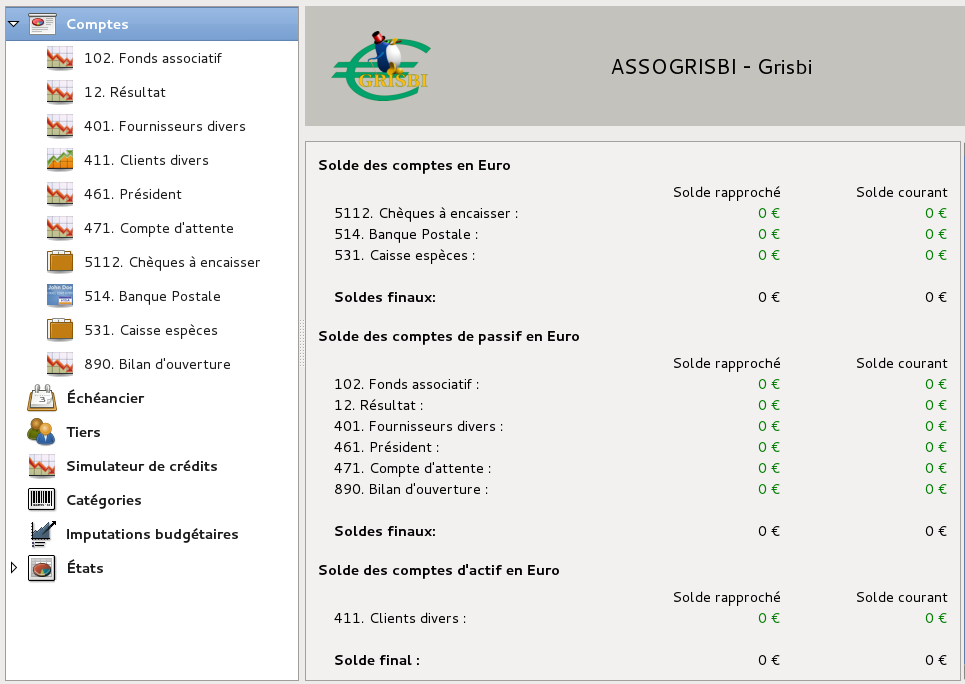
\includegraphics[scale=0.5]{image/screenshot/asso_account_creation}
\end{center}
\caption{Page d'accueil après création de tous les comptes}
\label{asso-account-creation-img}
\end{figure}
% image centrée
\fi

\ifIllustration
% saut de page pour titre solidaire
\newpage
\fi


\subsection{Reprise d'une comptabilité dans Grisbi\label{association-plan-opening}}
 
Pour reprendre la comptabilité déjà existante de votre association dans Grisbi, procédez comme suit :

\begin{enumerate}
	\item créez l'exercice de l'année en cours dans votre fichier de comptes (voir la section \vref{financialyear-start}, \menu{Mise en place des exercices}) ;
	\item dans le compte \menu{890.~Bilan d’Ouverture}, débitez de la somme des soldes de tous les comptes créditeurs en passant par une opération ventilée ;
	\item dans le compte \menu{890.~Bilan d’Ouverture}, créditez de la somme des soldes de tous les comptes débiteurs en passant par une opération ventilée.
\end{enumerate}	
				
À titre d'exemple, saisissez les soldes des comptes de bilan à la date du jour de la saisie (théoriquement le 1er jour de l’exercice) :
\begin{itemize}
	\item un solde bancaire de 300 ;
	\item un solde de 50 dans la caisse espèces ;
	\item plusieurs chèques d’un total de 150 à encaisser ;
	\item un solde du Fonds associatif de 350 ;
	\item une dette de 80 due au Président pour un achat effectué par lui pour l’association ;
	\item le résultat de l'exercice précédent de 70.			
\end{itemize}

% espace avant Attention ou Note : 5 mm
\vspacepdf{5mm}
\textbf{Note} : aucun résultat n'est destiné à rester durablement au compte \menu{12.~Résultat}, qui devra alors être apuré selon les décisions de l'assemblée générale. En attendant, il peut être facultativement viré au compte \menu{88.~Résultat en instance d’affectation}.

% espace pour changement de thème
\vspacepdf{5mm}
\ifIllustration Une fois ces opérations saisies, le compte \menu{890.~Bilan d'ouverture}\refimage{asso-renew-img} et la page d'accueil\refimage{asso-afterOpening-img}  devraient se présenter ainsi :
\else Une fois ces opérations saisies, vous pouvez consulter le compte \menu{890.~Bilan d'ouverture} et la page d'accueil de Grisbi.
\fi 

\ifIllustration
% image centrée
\begin{figure}[ht]
\begin{center}
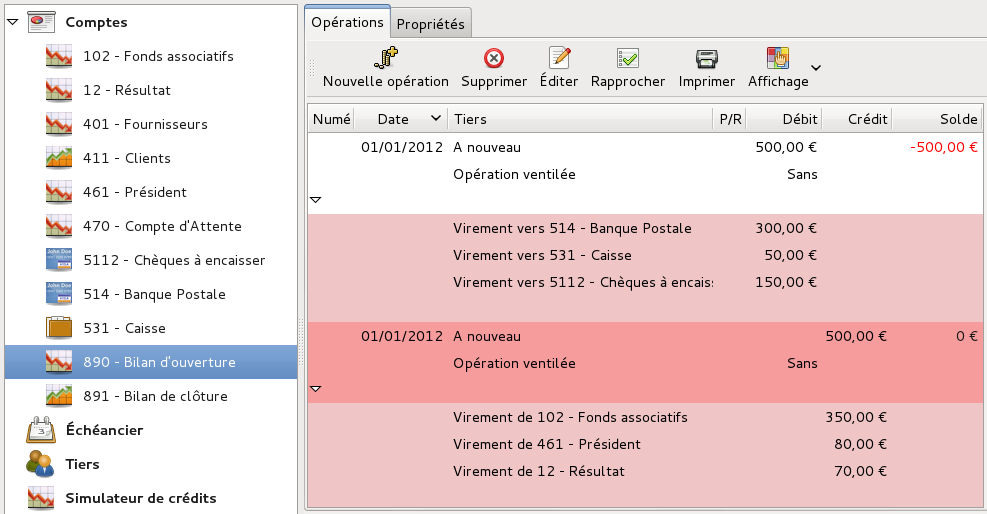
\includegraphics[scale=0.5]{image/screenshot/asso_renew}
\end{center}
\caption{Bilan d’ouverture : reprise des \og À nouveaux \fg{}}
\label{asso-renew-img}
\end{figure}
% image centrée
\fi

\ifIllustration
% image centrée
\begin{figure}[ht]
\begin{center}
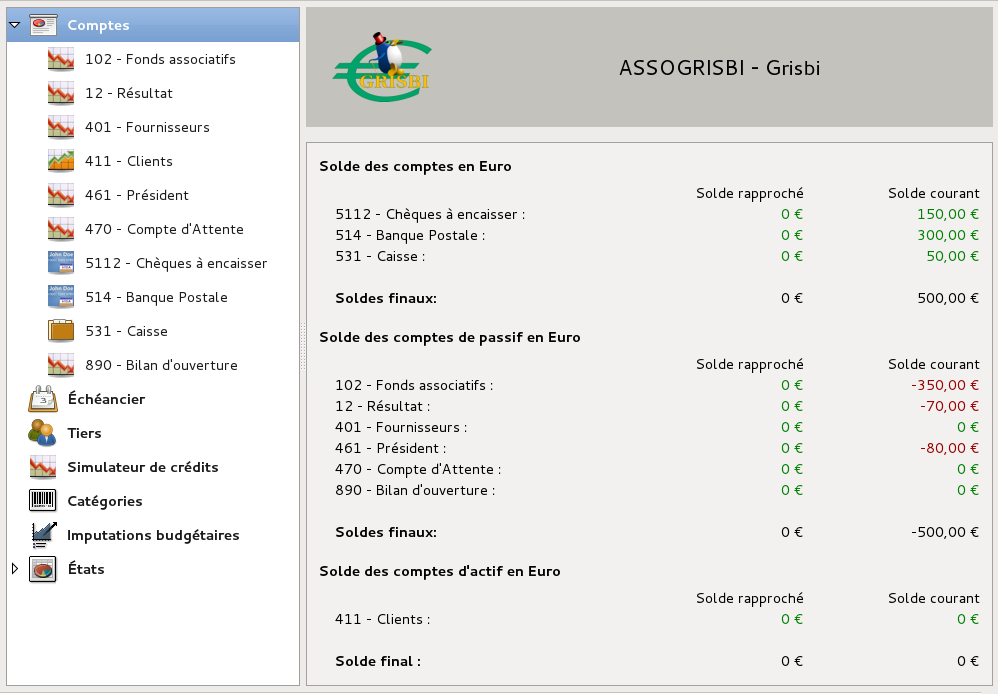
\includegraphics[scale=0.5]{image/screenshot/asso_afterOpening}
\end{center}
\caption{Page d'accueil après bilan d'ouverture}
\label{asso-afterOpening-img}
\end{figure}
% image centrée
\fi


\subsection{Mouvements entre comptes\label{association-plan-activity}}

Les mouvements entre comptes se font comme pour une comptabilité personnelle. Voici quelques exemples d'écritures courantes dans la comptabilité d'une association ou d'une petite entreprise (sans TVA) :

\begin{enumerate}
	\item facture d'achat ou de frais payée comptant : une seule écriture suffit pour comptabiliser le flux économique et le flux financier ; par exemple, achat de 80 € de carburant auto :
		\begin{itemize}
			\item sur le compte \menu{514.~Banque Postale},
			\item \menu{Débit} : 80 €,					
			\item \menu{Tiers} : nom du fournisseur,
			\item \menu{Catégorie} : 606.~Achats non stockés de matières et fournitures,
			\item \menu{Remarques} : numéro de la facture ;
		\end{itemize}
	\item facture d'achat ou de frais payée à crédit : deux écritures sont nécessaires :
		\begin{itemize}
			\item pour comptabiliser le flux économique (l'achat) :
				\begin{itemize}
					\item sur le compte \menu{401.~Fournisseurs divers},
					\item \menu{Débit} : 80 €,					
					\item \menu{Tiers} : nom du fournisseur,
					\item \menu{Catégorie} : 606.~Achats non stockés de matières et fournitures,
					\item \menu{Remarques} : numéro de la facture ;
				\end{itemize}			
			\item pour comptabiliser le flux financier (le paiement) :
				\begin{itemize}
					\item sur le compte \menu{514.~Banque Postale},
					\item \menu{Débit} : 80 €,					
					\item \menu{Tiers} : nom du fournisseur,
					\item \menu{Catégorie} : Virement : 401.~Fournisseurs,
					\item \menu{\No chèque/virement} : numéro du chèque ou du virement ;
				\end{itemize}
		\end{itemize}	
	\item vente au comptant ; sur le même principe, pour une vente dans une petite entreprise non assujettie à la TVA :
		\begin{itemize}
			\item sur le compte \menu{5112.~Chèques à encaisser},
			\item \menu{Crédit} : 80 €,					
			\item \menu{Tiers} : nom du client,
			\item \menu{Catégorie} : 707.~Ventes de marchandises (par exemple),
			\item \menu{Remarques} : numéro de la facture ;
		\end{itemize}						
	\item remise des chèques des clients à la banque :
		\begin{itemize}
			\item sur le compte \menu{514.~Banque Postale},
			\item \menu{Crédit} : 80 € (ou plus, avec éventuellement d’autres chèques),					
			\item \menu{Tiers} : Bordereau de remise n° xxxx,
			\item \menu{Catégorie} : Virement 5112.~Chèques à encaisser.
		\end{itemize}		
\end{enumerate}

%espace pour changement de thème
\vspacepdf{5mm}
Maintenant, un autre petit exercice : \emph{comment comptabiliser une vente à crédit (3 écritures) ?} Vous trouverez la réponse en fin de chapitre (voir le paragraphe \vref{association-answer-2}, \menu{Exercice 2}).


\subsection{Comptabilité analytique\label{association-plan-analytic}}

La comptabilité générale classe les charges et les produits par nature. Pour une association, il peut être nécessaire de tenir une comptabilité analytique qui classe recettes et dépenses (charges et produits) par destination ou par fonction. Il y a deux grandes classes :

\begin{itemize}
	\item la classe \emph{Gestion générale}, qui permet d'appréhender les frais généraux de l'association ;
	\item la classe \emph{Activités}, qui permet d'appréhender les coûts des diverses manifestations organisées.
\end{itemize}

Dans Grisbi, cette double imputation peut être traitée en utilisant les \menu{Imputations budgétaires}. Vous numéroterez ces imputations budgétaires en utilisant la classe 9 qui est disponible, et en créant deux blocs de sous-classes :

\begin{itemize}
	\item 91 à 94 pour la \emph{Gestion Générale} ;
	\item 95 à 99 pour les \emph{Activités}.
\end{itemize}

% espace pour changement de thème
\vspacepdf{5mm}
Voici deux exemples de tels mouvements :

\begin{enumerate}
	\item dépense de gestion générale pour l'achat de fournitures \ifIllustration informatiques\refimage{asso-ink-expense-img} :
	\else informatiques :
	\fi 
		\begin{itemize}
			\item sur le compte \menu{514.~Banque Postale} et par chèque,		
			\item \menu{Débit} : 60 €,					
			\item \menu{Tiers} : Bureau Tique,
			\item \menu{Catégorie} : 60 Achats (sauf 603) : 6064.~Fourniture administratives,
			\item \menu{Imputation} : 91.~Gestion Générale,
			\item \menu{Exercice} : 2012,
			\item \menu{Remarques} : Cartouches d'encre ;
		\end{itemize}

\ifIllustration
% image centrée
\begin{figure}[ht]
\begin{center}
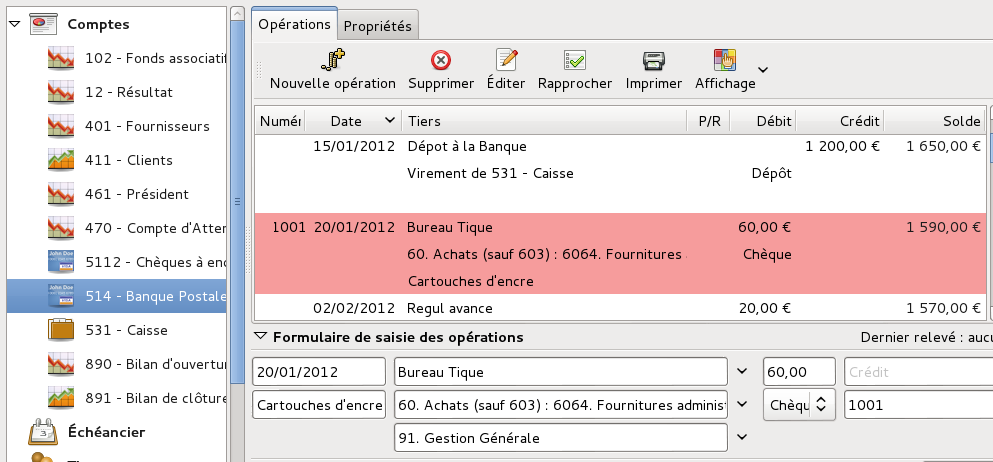
\includegraphics[scale=0.48]{image/screenshot/asso_ink_expense}
\end{center}
\caption{Saisie d'une opération d'achat de cartouches d'encre}
\label{asso-ink-expense-img}
\end{figure}
% image centrée
\fi

\ifIllustration
% saut de page pour texte solidaire
\newpage
\fi

	\item dépense pour l'achat de boisson pour la manifestation \ifIllustration Activité~2\refimage{asso-drink-expense-img} :
	\else Activité~2 :
	\fi
		\begin{itemize}
			\item sur le compte \menu{514.~Banque Postale} et par chèque,
			\item \menu{Débit} : 300 €,					
			\item \menu{Tiers} : Truc Enplume,
			\item \menu{Catégorie} : 60.~Achats (sauf 603) : 6070.~Achats de marchandises,
			\item \menu{Imputation} : 96.~Manifestation : 962.~Activité~2,
			\item \menu{Exercice} : 2012,
			\item \menu{Remarques} : Achat de boissons.
		\end{itemize}
\end{enumerate}

\ifIllustration
% image centrée
\begin{figure}[hb]
\begin{center}
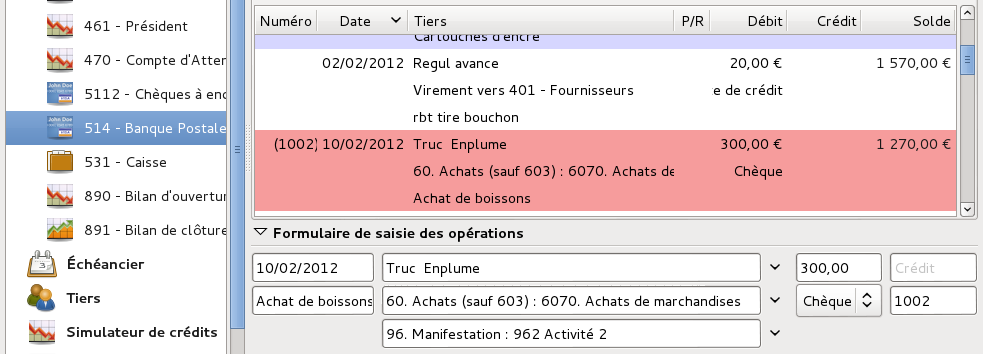
\includegraphics[scale=0.5]{image/screenshot/asso_drink_expense}
\end{center}
\caption{Saisie d'une opération d'achat de boissons pour la manifestation Activité~2}
\label{asso-drink-expense-img}
\end{figure}
% image centrée
\fi	

Vous pourrez en tirer des états plus ou moins détaillés, à vous de les créer suivant vos \ifIllustration besoins, par exemple\refimage{asso-analyticExpenses-img} :
	\else besoins.
	\fi
	
\ifIllustration
% image centrée
\begin{figure}[!ht]
\begin{center}
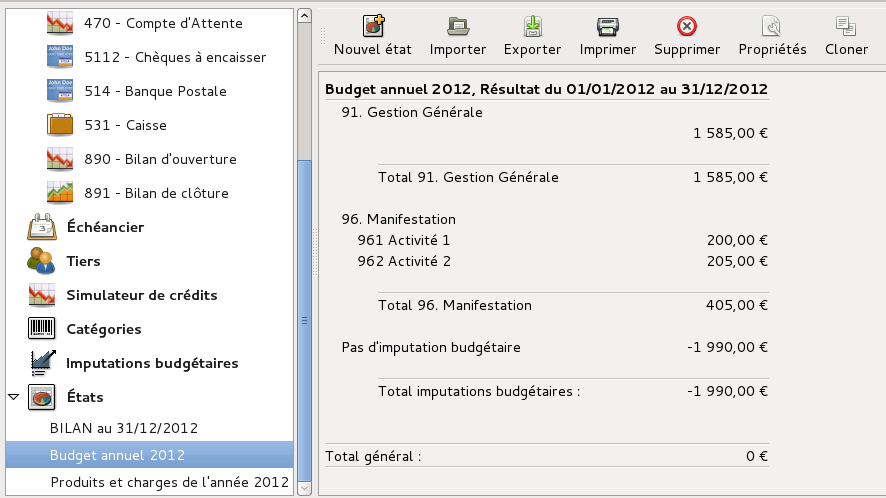
\includegraphics[scale=0.5]{image/screenshot/asso_analyticExpenses}
\end{center}
\caption{État détaillé des dépenses analytiques de Gestion générale et Activités}
\label{asso-analyticExpenses-img}
\end{figure}
% image centrée
\fi	

\ifIllustration
% saut de page pour titre solidaire
\newpage
\fi


\subsection {Travaux de fin d’exercice} \label{association-plan-closingWork}

En fin d'exercice, un certain nombre d'opérations doivent être comptabilisées ; voici quelques exemples :


\subsubsection {Dépréciation des biens immobilisés} 

Constatez la dépréciation des biens immobilisés dont l’association ou la petite entreprise est propriétaire ; par exemple pour l'amortissement d'un ordinateur de bureau acheté 500 euros sur 5 ans :
\begin{enumerate}
	\item créez le compte \menu{28183.~Amortissement matériel de bureau et informatique} ;		
	\item sur ce compte ;
	\item \menu{Débit} : 100 € (correspondant à 500/5) ;
	\item \menu{Tiers} : Amortissement matériel informatique ;
	\item \menu{Catégorie} : 681.~Dotation aux amortissements - Charges d'exploitation.
\end{enumerate}

Vous devrez comptabiliser cette opération chaque année pendant 5 ans. Si vous avez acheté le bien en cours d’année, vous devrez faire un calcul au prorata temporis pour la 1ère année.


\subsubsection {Comptabilisation des stocks}

\begin{enumerate}
	\item annulation du stock initial (stock à la fin de l’exercice précédent) :
		\begin{itemize}
			\item créez le compte \menu{370.~Stock de marchandises},		
			\item sur ce compte,
			\item \menu{Débit} : montant du stock initial,					
			\item \menu{Tiers} : Annulation stock initial,
			\item \menu{Catégorie} : 6037.~Variation de stocks de marchandises ;
		\end{itemize}
	\item enregistrement du stock final :
		\begin{itemize}
			\item sur le compte \menu{370.~Stock de marchandises},
			\item \menu{Crédit} : montant du stock final (suivant inventaire),					
			\item \menu{Tiers} : Enregistrement stock final,
			\item \menu{Catégorie} : 6037.~Variation de stocks de marchandises.
		\end{itemize}				
\end{enumerate}

\textbf{Note} : pour tout ce qui concerne les écritures de régularisation de fin d'exercice (charges à payer, charges constatées d'avance, etc.), qui assurent le respect de l'indépendance des exercices, consultez la documentation comptable mentionnée dans la section \vref{association-intro}, \menu{Introduction à la comptabilité d'association}.


\subsection {Documents de synthèse} \label{association-plan-synthesis}

Lors de la clôture d'un exercice, vous devez créer un certain nombre d'états. En particulier, trois états doivent être obligatoirement présentés lors de l'assemblée générale de l'association, qui est en charge d'approuver les comptes de l'exercice ; ce sont :

\begin{itemize}
	\item la Situation patrimoniale (Bilan) en fin d'exercice, présentée selon deux colonnes, Actif et Passif ;
	\item les Produits et Charges (Résultat) de l'exercice, qui est un résumé des mouvements Charges, enregistrés dans les comptes de classe 6, et des mouvements Produits, enregistrés dans les comptes de classe 7 ;
	\item la Comptabilité Analytique, qui est une synthèse des Produits et Charges par nature, enregistrés dans les comptes de classe 9, si cette fonction est tenue dans la comptabilité.
\end{itemize}

% espace avant Attention ou Note : 5 mm
\vspacepdf{5mm}
\textbf{Note} : pour \og Produits et Charges \fg {}, on parle très fréquemment dans les associations de \og Dépenses et Recettes \fg{} ; comme vous ne pouvez savoir si les documents comptables devront un jour être approuvés par un Commissaire aux comptes ou être présentés à une administration, il est conseillé d'anticiper cela, donc d'utiliser tout de suite le terme Produits et Charges, et ceci dès la création d'une comptabilité d'association. 
% espace après Attention ou Note : 5 mm
\vspacepdf{5mm}

Par ailleurs, Grisbi permet de créer des états préparatoires synthétiques de toutes sortes ; pour cela, consultez les chapitres :
\begin{itemize}
	\item \vref{reports}, \menu{États} ;
	\item \vref{reportscreation}, \menu{Création d'un état}.
\end{itemize}


\subsection {Paramétrage des états synthétiques de clôture d'un exercice\label{association-plan-synthesis-parameters}}

Pour configurer chacun des trois états, suivez la procédure de création à partir de la section \vref{reportscreation-start}, \menu{Choix du modèle de l'état de départ}. Ajustez, dans la fenêtre de création/modification des états, les paramètres communs et les paramètres spécifiques à cet état, comme indiqué ci-dessous ; une fois chaque configuration terminée et validée, l'état concerné apparaîtra sous l'onglet \menu{États} du panneau de navigation de Grisbi.


\subsubsection {Paramètres communs à ces trois états :}

\begin{itemize}
	\item \menu{Dates} :
		\begin{itemize}
			\item cochez \menu{Utiliser les exercices},
% saut de ligne pour indentation correcte de la note dans la liste

			\vspacepdf{2mm}
			\textbf{Note} : pour pouvoir utiliser des exercices, il faut que ceux-ci soient configurés dans le menu \menu{Édition - Préférences} (voir la section \vref{financialyear-start}, \menu{Mise en place des exercices}).
			\item cochez \menu{Détailler les exercices utilisés},
			\item sélectionnez l'exercice voulu dans la liste juste en-dessous ;
		\end{itemize}
	\item \menu{Virements} : cochez \menu{Inclure les virements de ou vers les comptes} et choisissez \menu{Sélectionner tout} ;
	\item \menu{Comptes} : choisissez \menu{Sélectionner tout} ;
	\item \menu{Tiers} : choisissez \menu{Sélectionner tout} ;
	\item \menu{Catégories} : choisissez \menu{Sélectionner tout} ;
	\item \menu{Imputations budgétaires} : choisissez \menu{Sélectionner tout} ;
	\item \menu{Modes de règlement} : choisissez \menu{Sélectionner tout} ;
	\item \menu{Divers} : cochez \menu{Sélectionner toutes les opérations}.		
\end{itemize}	

		
\subsubsection {Paramètres pour l'état Situation patrimoniale (Bilan) :}		
			
\begin{itemize}
	\item \menu{Groupement des données} :
		\begin{itemize}
			\item cochez \menu{Regrouper les opérations par compte},				
			\item dans le tableau, faites monter le libellé \menu{Compte} en tête ;
		\end{itemize}					
	\item \menu{Séparation des données} : ne rien cocher ;			
	\item \menu{Généralités} :
		\begin{itemize}
			\item \menu{Nom de l'état} : saisissez un nom, sachant que cet état correspond au bilan au jj/mm/aa ; 
		\end{itemize}									
	\item \menu{Titres} : dans la zone \menu{Comptes}, cocher \menu{Afficher le nom du compte} et \menu{Afficher un sous-total lors d'un changement de compte} ;
	\item \menu{Opérations} : ne pas cocher \menu{Afficher les opérations}.
\end{itemize}

		
\subsubsection {Paramètres pour l'état Produits et Charges de l'exercice (Résultat) :}		
			
\begin{itemize}
	\item \menu{Groupement des données} :
		\begin{itemize}
			\item cochez \menu{Regrouper les opérations par catégorie},				
			\item dans le tableau, faites monter le libellé \menu{Catégorie} en tête ;
		\end{itemize}					
	\item \menu{Séparation des données} : cochez \menu{Séparer les revenus et les dépenses} ;			
	\item \menu{Généralités} :
		\begin{itemize}
			\item \menu{Nom de l'état} : saisissez un nom, par exemple \og Revenus et dépenses de l'exercice xxxx \fg{} ou, de préférence, \og Produits et Charges de l'exercice xxxx \fg{} ; 
		\end{itemize}									
	\item \menu{Titres} : dans la zone \menu{Catégories}, cochez toutes les cinq cases ;
	\item \menu{Opérations} : ne pas cocher \menu{Afficher les opérations}.							
\end{itemize}

		
\subsubsection {Paramètres pour l'état Comptabilité Analytique :}
		
\begin{itemize}			
	\item \menu{Groupement des données} :
		\begin{itemize}
			\item cochez \menu{Regrouper les opérations par imputation budgétaire},				
			\item dans le tableau, faites monter le libellé \menu{Imputation budgétaire} en tête ;
		\end{itemize}					
	\item \menu{Séparation des données} : ne rien cocher ;			
	\item \menu{Généralités} :
		\begin{itemize}
			\item \menu{Nom de l'état} : saisissez un nom, par exemple \og Comptabilité analytique exercice xxxx \fg{} ;
		\end{itemize}									 
	\item \menu{Titres} : dans la zone \menu{Imputations budgétaires}, cochez les quatre premières cases, mais pas la case \menu{Afficher \og Pas de sous-imputation si absente\fg{}}.			
\end{itemize}		
 
\ifIllustration
% saut de page pour titre solidaire
\newpage
\fi


\subsection {Clôture d'un exercice\label{association-plan-closingResult}}

Grisbi ne dispose pas de la fonction de clôture automatique en fin d'exercice comptable. Cela ne doit pas empêcher le respect des règles du PCG (Plan Comptable Général) Art. 441/12, ce qui peut sembler un peu fastidieux, mais cela ne se produit qu'une fois par an\ldots{} Les sections suivantes indiquent comment procéder :


\subsubsection {Solde des comptes de produits et charges, Résultat et Bilan :}

Pour solder les comptes de produits et charges, il faut les virer au compte \menu{12.~Résultat} ; procédez comme suit :

\begin{enumerate}
	\item imprimez l'état Produits et Charges de l'exercice afin d'obtenir le solde de chaque compte des classes 6 et 7 \ifIllustration \refimage{asso-chargesProducts-img}
	\else
	\fi (au besoin, voir la section \vref{association-plan-synthesis-parameters}, \menu{Paramétrage des états synthétiques de clôture d'un exercice}) ;

\ifIllustration
% image centrée
\begin{figure}[p]
\begin{center}
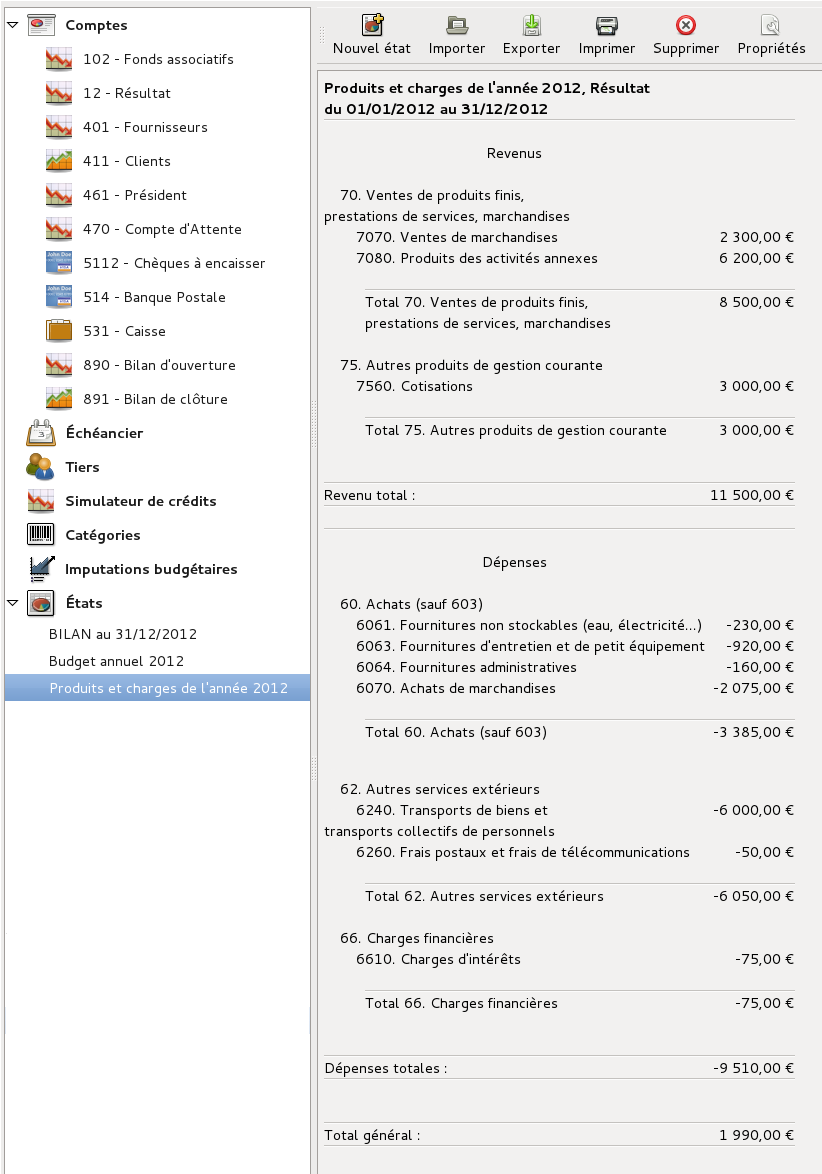
\includegraphics[scale=0.5]{image/screenshot/asso_chargesProducts}
\end{center}
\caption{État Produits et Charges de l'exercice (Résultat)}
\label{asso-chargesProducts-img}
\end{figure}
% image centrée
\fi

	\item faites un virement de tous les comptes de charges au compte \menu{12.~Résultat} :
		\begin{itemize}
			\item sur le compte \menu{12.~Résultat},
			\item \menu{Crédit} : somme des soldes des comptes de la classe 6 (charges),					
			\item \menu{Tiers} : Virement des comptes de charges à Résultat,
			\item \menu{Catégorie} : Opération ventilée : ventiler le solde de tous les comptes de la classe 6 (charges) ;
		\end{itemize}			
	\item faites un virement de tous les comptes de produits au compte \menu{12.~Résultat} :
		\begin{itemize}
			\item sur le compte \menu{12.~Résultat},
			\item \menu{Débit} : somme des  soldes des comptes de la classe 7 (produits),					
			\item \menu{Tiers} : Virement des comptes de produits à Résultat,
			\item \menu{Catégorie} : Opération ventilée : ventiler le solde de tous les comptes de la classe 7 (produits) ;
		\end{itemize}	
	\item constatez le solde du compte \menu{12.~Résultat} \ifIllustration \refimage{asso-chargesProductsClosing-img}; 
	\else ;
	\fi  

\ifIllustration
% image centrée
\begin{figure}[p]
\begin{center}
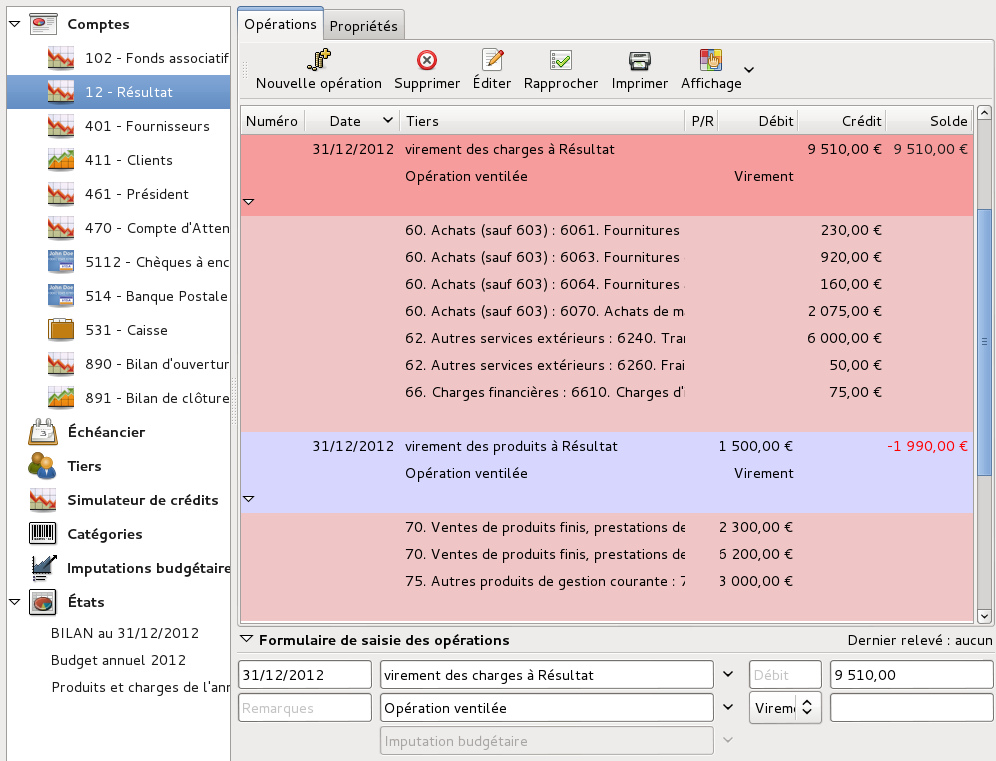
\includegraphics[scale=0.5]{image/screenshot/asso_chargesProductsClosing}
\end{center}
\caption{Clôture des comptes de produits et charges et détermination du résultat de l'exercice}
\label{asso-chargesProductsClosing-img}
\end{figure}
% image centrée
\fi


	\item vérifiez que les soldes des comptes de produits et charges sont égaux à zéro à la fin de l'exercice et que tout est regroupé dans le compte \menu{12.~Résultat} ; le solde du compte Résultat représente le bénéfice ou les pertes de l'exercice ;
	\item imprimez enfin le \ifIllustration bilan de l'exercice\refimage{asso-balanceSheet-img}.
	\else bilan de l'exercice.
	\fi
\end{enumerate}

\ifIllustration
% image centrée
\begin{figure}[p]
\begin{center}
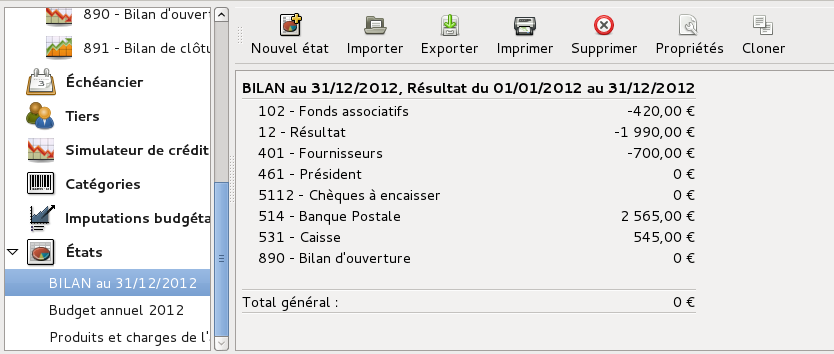
\includegraphics[scale=0.5]{image/screenshot/asso_balanceSheet}
\end{center}
\caption{État Situation patrimoniale (Bilan)}
\label{asso-balanceSheet-img}
\end{figure}
% image centrée
\fi

\ifIllustration
% saut de page pour titre solidaire
\newpage
\newpage
\newpage
\fi


\subsubsection {Clôture et réouverture des comptes :}

Ces écritures permettent le report des soldes des comptes de bilan sur l'exercice suivant (À nouveau).

\begin{enumerate}
	\item  clôture des comptes d'actif \ifIllustration \refimage{asso-accounts-closing-img} :
	\else :
	\fi
		\begin{itemize}
			\item sur le compte \menu{891.~Bilan de clôture},
			\item \menu{Crédit} : somme des comptes d'actif (ils apparaissent en positif sur l'état \og Situation patrimoniale \fg{}),
			\item \menu{Tiers} : Clôture des comptes d'actif,
			\item \menu{Catégorie} : \menu{Opération ventilée} : ventiler les soldes de tous les comptes d'actif ;
		\end{itemize}
	\item clôture des comptes de passif \ifIllustration \refimage{asso-accounts-closing-img} :
	\else :
	\fi
		\begin{itemize}
			\item sur le compte \menu{891.~Bilan de clôture},
			\item \menu{Date} : date de fin d'exercice,
			\item \menu{Débit} : somme des soldes des comptes de passif (ils apparaissent en négatif sur l'état \og Situation patrimoniale \fg{}),
			\item \menu{Tiers} : Clôture comptes de passif,
			\item \menu{Catégorie} : \menu{Opération ventilée} : ventiler les soldes de tous les comptes de passif ;
		\end{itemize}

		\ifIllustration
		% image centrée
		\begin{figure}[!ht]
		\begin{center}
		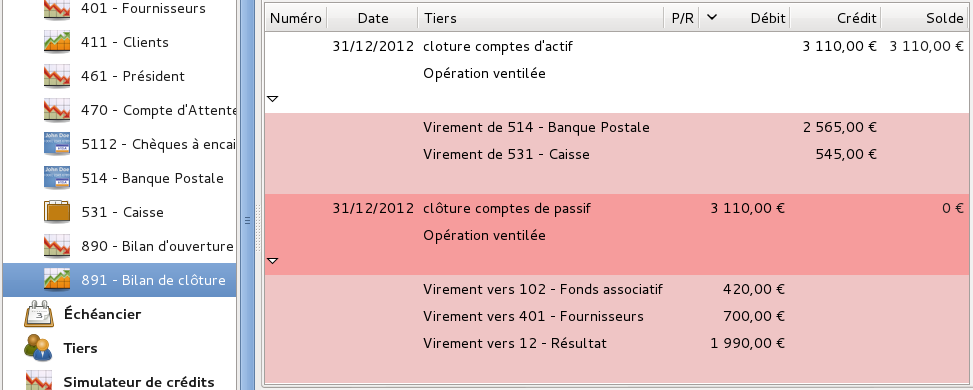
\includegraphics[scale=0.5]{image/screenshot/asso_accounts_closing}
		\end{center}
		\caption{Clôture des comptes d'actif et de passif}
		\label{asso-accounts-closing-img}
		\end{figure}
		% image centrée
		\fi

	\item réouverture des comptes d'actif au début de l'exercice suivant \ifIllustration \refimage{asso-accounts-reopening-img} :
	\else :
	\fi
		\begin{itemize}
			\item sur le compte \menu{890.~Bilan d'ouverture},
			\item \menu{Débit} : somme des soldes des comptes d'actif (ils apparaissent en positif),
			\item \menu{Tiers} : Ouverture des comptes d'actif,
			\item \menu{Catégorie} : \menu{Opération ventilée} : ventiler les soldes de tous les comptes d'actif ;
		\end{itemize}		
	\item réouverture des comptes de passif au début de l'exercice suivant \ifIllustration \refimage{asso-accounts-reopening-img} :
	\else :
	\fi
		\begin{itemize}
			\item sur le compte \menu{890.~Bilan d'ouverture},
			\item \menu{Date} : date de début de l'exercice suivant,
			\item \menu{Crédit} : somme des soldes des comptes de passif,
			\item \menu{Tiers} : Ouverture des comptes de passif,
			\item \menu{Catégorie} : \menu{Opération ventilée} : ventiler les soldes de tous les comptes de passif ;
		\end{itemize}
	\item vous pourrez alors archiver les opérations de l'exercice passé, qui restent consultables, mais qui ne devront jamais plus être modifiées, pour assurer l'intangibilité et l'irréversibilité des informations.
\end{enumerate}		

		\ifIllustration
		% image centrée
		\begin{figure}[!ht]
		\begin{center}
		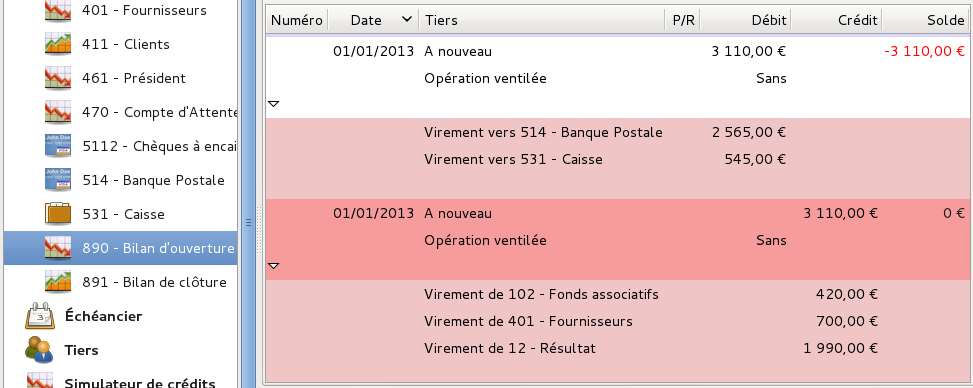
\includegraphics[scale=0.5]{image/screenshot/asso_accounts_reopening}
		\end{center}
		\caption{Réouverture des comptes d'actif et de passif}
		\label{asso-accounts-reopening-img}
		\end{figure}
		% image centrée
		\fi

\ifIllustration
% saut de page pour titre solidaire
\newpage
\fi

\strong{Attention} : Grisbi ne dispose pas de la fonction de clôture automatique en fin d'exercice comptable ; la conservation intégrale de vos données après la clôture d'un exercice n'est donc pas totalement assurée, car vous pourriez encore les modifier par inadvertance; il vous appartient de veiller à la pérennité de vos données, par exemple en faisant une copie de sauvegarde de votre fichier de comptes à la date de la fin de cet exercice.

\ifIllustration
% saut de page pour report page suivante
\newpage
\else
\fi


\section {Réponses aux exercices} \label{association-answer}

\paragraph{Exercice 1 :\label{association-answer-1} \emph{Hector Boyau a pris 10 bouteilles pour lui et demande donc qu'on ne lui rembourse que 150 euros. Comment enregistrez-vous cela ?}}

Hector Boyau avait acheté 60 bouteilles et 10 cubis pour 280 euros, l'opération d'achat avait été passée en opération ventilée (voir la section \vref{asso-simple-secondCase}, \menu{Deuxième cas de figure}) :

\begin{enumerate}
	\item achat de 10 bouteilles à l’association par Hector Boyau :
		\begin{itemize}
			\item sur le compte d'avances ; 
			\item \menu{Crédit} : 30 euros ;
			\item \menu{Tiers} : \emph{Hector Boyau} ;
			\item \menu{Catégorie} : \emph{Virement : Pinard en bouteilles} ;
			\item \menu{Remarques} : \emph{Achat de 10 bouteilles par Hector Boyau}.
		\end{itemize}
	\item remboursement à Hector Boyau :
		\begin{itemize}
			\item sur le compte bancaire ; 
			\item \menu{Débit} : 150 euros ;
			\item \menu{Tiers} : \emph{Remboursement Hector Boyau} ;
			\item \menu{Catégorie} : \emph{Virement : compte d’avances} ;
			\item \menu{Remarques} : \emph{Remboursement des 50 bouteilles à Hector Boyau}.
		\end{itemize}
\end{enumerate}

	
\paragraph{Exercice 2 :\label{association-answer-2} \emph{Comment comptabiliser une vente à crédit} ? Trois écritures sont nécessaires :}

\begin{enumerate}
	\item vente à crédit (flux économique) :
		\begin{itemize}
			\item sur le compte 411.~Clients,
			\item \menu{Crédit} : 80 €,					
			\item \menu{Tiers} : numéro de facture et nom du client,
			\item \menu{Catégorie} : 707.~Ventes de marchandises (par exemple)
		\end{itemize}				
	\item réception du chèque (flux financier) :
		\begin{itemize}
			\item sur le compte 5112.~Chèques à encaisser,
			\item \menu{Crédit} : 80 €,					
			\item \menu{Tiers} : nom du client,
			\item \menu{Catégorie} : Virement : 411.~Clients ;
		\end{itemize}
	\item remise des chèques des clients à la banque :
		\begin{itemize}
			\item sur le compte 512.~Compte bancaire,
			\item \menu{Crédit} : 80 € (ou plus, avec éventuellement d’autres chèques),				
			\item \menu{Tiers} : Bordereau de remise n° xxxx,
			\item \menu{Catégorie} : Virement 5112.~Chèques à encaisser ;
		\end{itemize}
\end{enumerate}



	
	
	
	
	

